\documentclass[a4paper]{article}
\usepackage[a4paper,margin=0mm]{geometry}
\usepackage{fontspec}
\usepackage{unicode-math}
\usepackage{tikz}
\usetikzlibrary{fit,calc,positioning,arrows.meta}
\usepackage[table]{xcolor}
\usepackage[absolute]{textpos}
\usepackage{array}

\setmainfont{Libertinus Serif}
\setsansfont{Libertinus Sans}
\setmathfont{Libertinus Math}

\definecolor{accent}{HTML}{602785}
\definecolor{badge}{HTML}{B8A0C8}
\definecolor{ink}{HTML}{2A2E30}

\setlength{\TPHorizModule}{1mm}
\setlength{\TPVertModule}{1mm}
\setlength{\parindent}{0pt}
\pagestyle{empty}

\newcommand{\topicheader}[2]{%
\begin{textblock*}{194mm}(16mm,10mm)
\begin{tikzpicture}
\node[fill=accent,text=white,font=\sffamily\bfseries\fontsize{13}{13}\selectfont,
      minimum width=9mm,minimum height=9mm,inner sep=0pt] at (4.5mm,-4.5mm) {#1};
\node[font=\sffamily\bfseries\fontsize{15}{16}\selectfont,text=ink,anchor=west] at (12mm,-4.5mm) {#2};
\end{tikzpicture}
\end{textblock*}
\begin{textblock*}{194mm}(16mm,22.5mm)

\begin{tikzpicture}
\fill[accent] (0,0) rectangle (194mm,0.5mm);
\end{tikzpicture}
\end{textblock*}
}

\newcommand{\pagekicker}[1]{%
\begin{textblock*}{100mm}(16mm,25.5mm)
\begin{tikzpicture}
\node[fill=ink,text=white,font=\sffamily\bfseries\fontsize{8}{8}\selectfont,
      inner sep=2.2pt,rounded corners=1pt] {\MakeUppercase{#1}};
\end{tikzpicture}
\end{textblock*}
}

\newcommand{\videobanner}[1]{%
\begin{textblock*}{178mm}(16mm,25.5mm)
\begin{tikzpicture}
\fill[accent] (0,0) rectangle (178mm,-10mm);
\draw[white,line width=0.6pt] (3mm,-1.7mm) rectangle (11.5mm,-8.3mm);
\node[white,font=\sffamily\fontsize{4}{4.4}\selectfont,align=center] at (7.25mm,-5mm) {QR\\CODE};
\node[white,font=\sffamily\bfseries\fontsize{9.5}{11}\selectfont,anchor=west] at (16mm,-5.6mm) {WATCH THE VIDEO BEFORE YOU SOLVE};
\node[white,font=\sffamily\fontsize{7.5}{8}\selectfont,anchor=east] at (174mm,-5.6mm) {YouTube ~\textbullet~ #1};
\end{tikzpicture}
\end{textblock*}
}

\newcommand{\pagefooter}[1]{%
\begin{textblock*}{194mm}(8mm,286.41mm)
  
\begin{tikzpicture}
    \fill[accent] (0,0) rectangle (194mm,0.6mm);
  \end{tikzpicture}
\end{textblock*}
\begin{textblock*}{63.59mm}(8mm,288.27mm)
  {\sffamily\bfseries\color{accent}\fontsize{13}{16}\selectfont SAT 1200+}
\end{textblock*}
\begin{textblock*}{10mm}(188mm,288.27mm)
  \centering{\sffamily\color{accent}\fontsize{14}{16}\selectfont #1}
\end{textblock*}
}

\newcommand{\cardbg}[4]{%
\begin{textblock*}{#3mm}(#1mm,#2mm)
\begin{tikzpicture}
\fill[badge!22,rounded corners=3mm] (0,0) rectangle (#3mm,-#4mm);
\end{tikzpicture}
\end{textblock*}%
}

\newcommand{\pill}[3]{%
\begin{textblock*}{160mm}(#1mm,#2mm)
\begin{tikzpicture}
\node[fill=accent,text=white,anchor=north west,font=\sffamily\bfseries\fontsize{10}{10}\selectfont,
      rounded corners=8pt,inner xsep=5mm,inner ysep=1.8mm] at (0,0) {RULE ~\textperiodcentered~ #3};
\end{tikzpicture}
\end{textblock*}%
}

\arrayrulecolor{accent}
\setlength{\arrayrulewidth}{0.7pt}
\renewcommand{\arraystretch}{1.5}

\begin{document}

% ======================================================================
% PAGE 1
% ======================================================================
\topicheader{23}{The Pythagorean Theorem \& Coordinates}
\videobanner{Lesson 23}
\pagefooter{123}
\mbox{}%

% ---- CARD 1: Pythagorean theorem ----
\cardbg{16}{40}{178}{95}
\pill{26}{43}{Pythagorean theorem (Pifagor teoremasi)}

\begin{textblock*}{85mm}(26mm,58mm)
{\fontsize{15}{18}\selectfont $a^2+b^2=c^2$}
\end{textblock*}

\begin{textblock*}{55mm}(140mm,58mm)
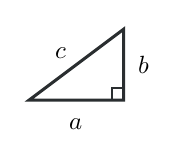
\begin{tikzpicture}
\draw[ink,line width=1.1pt] (0,0) -- (12mm,0) -- (12mm,9mm) -- cycle;
\draw[ink,line width=0.8pt] (12mm,0) -- (10.5mm,0) -- (10.5mm,1.5mm) -- (12mm,1.5mm);
\node[font=\fontsize{9}{9}\selectfont] at (6mm,-3mm) {$a$};
\node[font=\fontsize{9}{9}\selectfont] at (14.5mm,4.5mm) {$b$};
\node[font=\fontsize{9}{9}\selectfont] at (4mm,6mm) {$c$};
\end{tikzpicture}
\end{textblock*}

\begin{textblock*}{158mm}(26mm,80mm)
{\fontsize{10.5}{13}\selectfont\color{ink}
Legs $a,b$ meet at the right angle; hypotenuse $c$ is opposite it and always
the longest side. Only applies when that right angle is marked or given --
SAT figures aren't always drawn to scale.}
\end{textblock*}

\begin{textblock*}{158mm}(26mm,110mm)
{\fontsize{13}{16}\selectfont
$a=9,\ b=12\colon\ 9^2+12^2=81+144=225\ \Longrightarrow\ c=\sqrt{225}=15$}
\end{textblock*}

% ---- CARD 2: Identify the hypotenuse first ----
\cardbg{16}{143}{178}{45}
\pill{26}{146}{Identify the hypotenuse first}

\begin{textblock*}{158mm}(26mm,160mm)
{\fontsize{10.5}{13}\selectfont\color{ink}
An unknown side isn't always the hypotenuse -- it may be a leg. Write the
formula with $c$ in the right place.}
\end{textblock*}

\begin{textblock*}{158mm}(26mm,173mm)
{\fontsize{12}{15}\selectfont
Hyp.\ $=13$, leg $=5$: $\ 5^2+x^2=13^2\ \Longrightarrow\ x=\sqrt{169-25}=12$}
\end{textblock*}

\clearpage

% ======================================================================
% PAGE 2
% ======================================================================
\topicheader{23}{The Pythagorean Theorem \& Coordinates}
\pagekicker{Rules sheet -- 2/2}
\pagefooter{124}
\mbox{}%

% ---- CARD 3: Distance formula ----
\cardbg{16}{33}{178}{92}
\pill{26}{36}{Distance formula (masofa formulasi)}

\begin{textblock*}{80mm}(26mm,51mm)
{\fontsize{13}{16}\selectfont $d=\sqrt{(x_2-x_1)^2+(y_2-y_1)^2}$}
\end{textblock*}

\begin{textblock*}{60mm}(130mm,49mm)
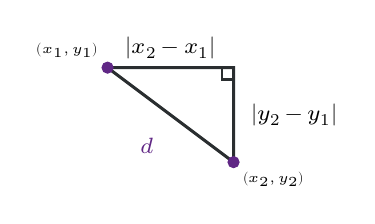
\begin{tikzpicture}
\draw[ink,line width=1.1pt] (0,10mm) -- (16mm,10mm) -- (16mm,-2mm) -- cycle;
\draw[ink,line width=0.8pt] (16mm,10mm) -- (14.5mm,10mm) -- (14.5mm,8.5mm) -- (16mm,8.5mm);
\filldraw[accent] (0,10mm) circle (0.7mm);
\filldraw[accent] (16mm,-2mm) circle (0.7mm);
\node[font=\tiny,anchor=south east] at (0,10mm) {$(x_1,y_1)$};
\node[font=\tiny,anchor=north west] at (16mm,-2mm) {$(x_2,y_2)$};
\node[font=\fontsize{8}{8}\selectfont] at (8mm,12.5mm) {$|x_2-x_1|$};
\node[font=\fontsize{8}{8}\selectfont,anchor=west] at (17mm,4mm) {$|y_2-y_1|$};
\node[font=\fontsize{8}{8}\selectfont,text=accent] at (5mm,0mm) {$d$};
\end{tikzpicture}
\end{textblock*}

\begin{textblock*}{158mm}(26mm,80mm)
{\fontsize{10.5}{13}\selectfont\color{ink}
This is just the Pythagorean theorem with the horizontal and vertical
legs built from the coordinates.}
\end{textblock*}

\begin{textblock*}{158mm}(26mm,93mm)
{\fontsize{13}{16}\selectfont
$(2,3),(7,15)\colon\ d=\sqrt{5^2+12^2}=\sqrt{169}=13$}
\end{textblock*}

\begin{textblock*}{158mm}(26mm,108mm)
{\fontsize{10}{13}\selectfont\color{black!55}\itshape
Each difference is squared, so a negative difference (e.g.\ $2-7=-5$) still
gives a positive result: $(-5)^2=25$.}
\end{textblock*}

% ---- CARD 4: Pythagorean triples ----
\cardbg{16}{131}{178}{80}
\pill{26}{134}{Common Pythagorean triples}

\begin{textblock*}{158mm}(26mm,148mm)
{\fontsize{10.5}{13}\selectfont
\begin{tabular}{|>{\centering\arraybackslash}p{30mm}|p{118mm}|}
\hline
\rowcolor{accent}
{\color{white}\textbf{Base triple}} & {\color{white}\textbf{Common multiples}} \\ \hline
$3,4,5$ & $6,8,10$\ \ $9,12,15$\ \ $12,16,20$ \\ \hline
$5,12,13$ & $10,24,26$ \\ \hline
$8,15,17$ & -- \\ \hline
$7,24,25$ & -- \\ \hline
\end{tabular}}
\end{textblock*}

\begin{textblock*}{158mm}(26mm,198mm)
{\fontsize{10}{13}\selectfont\color{black!55}\itshape
Not every right triangle's sides form a triple -- irrational results like
$\sqrt2$ or $\sqrt{10}$ are normal too.}
\end{textblock*}

\end{document}
